\section{What the decision should depend on}
\label{sec:depends}
\label{sec:analysis}

A decision should follow the question it is asked, the evidence it is given and the rubric it is told to
apply. Each subsection takes one of these inputs, shows how a natural design lets the decision drift away
from it, and gives the control that exposed the drift and the change that repaired it. Unless stated
otherwise, models here are 1.7B, trained for 12k steps on the evidence and knowledge mixture, and
$\dqsh$ is measured on the MMLU-Pro probe against the teacher's .102.

\subsection{The question}
\label{sec:analysis:deltaq}

The decision should change when the question changes. The design that fails this test is the one that is
cheaper to serve in throughput mode (\Cref{sec:results:cost}): a candidate-blind variant computes a
decision state $Z(\state, \query)$ before the candidates are seen, scores each candidate against it with
a learned head, and is distilled from the listwise teacher. Accuracy hides the gap because
candidate-blind states learn priors and calibration. Their accuracy of
.12--.17 sits above the .10 chance rate and comes from which option strings tend to be correct together (\Cref{app:extra-figures}).

$\dqsh$ exposes the failure. In every configuration we tested, question-conditioned capability appeared
only when the candidates were processed inside the forward pass. Six candidate-blind variants, spanning
three head factorizations, two distillation objectives and two tap depths, all have $\dqsh$ within .03
of zero, while N1, N3 and the teacher sit at .09--.12 and even N2 keeps .058 (\Cref{fig:deltaq};
per-variant numbers in \Cref{tab:blind}).

No lever we varied moves $\dqsh$, including cross-attention over all candidate tokens, multi-set
log-odds supervision and full-depth reading, though we cannot exclude optimization
(\Cref{app:extra-figures}). The question-dependent component lives in candidate-contextual computation, so Typical renders the candidates inside the backbone's
forward pass. Any architecture that scores candidates against a precomputed representation should report
$\dq$ alongside accuracy.

\label{sec:analysis:readout}
Rendering the candidates leaves open what the decision state is scored against. \Cref{tab:n1n3}
compares the readouts of \Cref{sec:method:readout} on one pass: letter logits (N1), $\hD$ against an
independent embedding of each option's text (N2), and $\hD$ against each option's contextual state
$\hctx{j}$ (N3). All arms render the candidates in the suffix, train on identical data with per-step
option shuffling, and read all 28 layers, so N2 and N3 differ only in what $\hD$ is scored against. The candidate's
contextual state carries the decision. N2 loses 10--12 points of among-$\numcands$
accuracy against N3 and 13 against N1, half of the question-conditioned signal ($\dqsh$ .058 vs.\ .106
for N3 across seeds), and collapses on Banking77 at $\numcands{=}77$ (.012). The pattern fits a decision
state that encodes which rendered slot holds the answer: the letter embedding and the contextual state
both carry slot identity, and an independently embedded label carries only its meaning. N3 matches N1 on
question dependence within seed noise: across seeds N1 averages $\dqsh = .109$ and N3 .106, within the
.01--.02 seed spread of both, and among-$\numcands$ accuracy is 1--2 points lower for N3. On evidence tasks N3 leads in
both seeds by 2 points on SNLI, 5.5--7 on MNLI and 4--5 on ANLI, and trails by 2--3 on BoolQ. N3 is the
readout Typical deploys.

\begin{figure}[t]
  \centering
  \begin{minipage}[t]{0.53\linewidth}
    \vspace{0pt}
    \captionof{table}{Three readouts of one decision pass, full-depth 1.7B backbone, identical data and
    steps; N1 and N3 at two seeds (\texttt{s0}/\texttt{s1}), N2 at one. Order measures are zero for a
    set-invariant scorer.}
    \label{tab:n1n3}
    \footnotesize
    \setlength{\tabcolsep}{2.5pt}
    \resizebox{\linewidth}{!}{%
    \begin{tabular}{lrrrrrr}
      \toprule
      & N1 s0 & N1 s1 & N2 & N3 s0 & N3 s1 & Teacher \\
      \midrule
      $\dqsh$ (primary) & .114 & .104 & .058 & .117 & .094 & .102 \\
      MMLU-Pro among-$\numcands$ & .325 & .318 & .198 & .314 & .301 & .310 \\
      Banking77, $\numcands{=}77$ & .531 & -- & .012 & .497 & -- & -- \\
      SNLI & .838 & .831 & .854 & .863 & .851 & -- \\
      MNLI & .684 & .664 & .742 & .752 & .719 & -- \\
      ANLI & .377 & .393 & .410 & .431 & .437 & -- \\
      BoolQ & .769 & .764 & .775 & .737 & .746 & -- \\
      Reorder $\Delta p$ & .165 & .165 & .059 & .101 & .109 & .097 \\
      Pairwise $\Delta$log-odds & .463 & .443 & .379 & .126 & .094 & .179 \\
      \bottomrule
    \end{tabular}}
  \end{minipage}\hfill
  \begin{minipage}[t]{0.44\linewidth}
    \vspace{0pt}
    \centering
    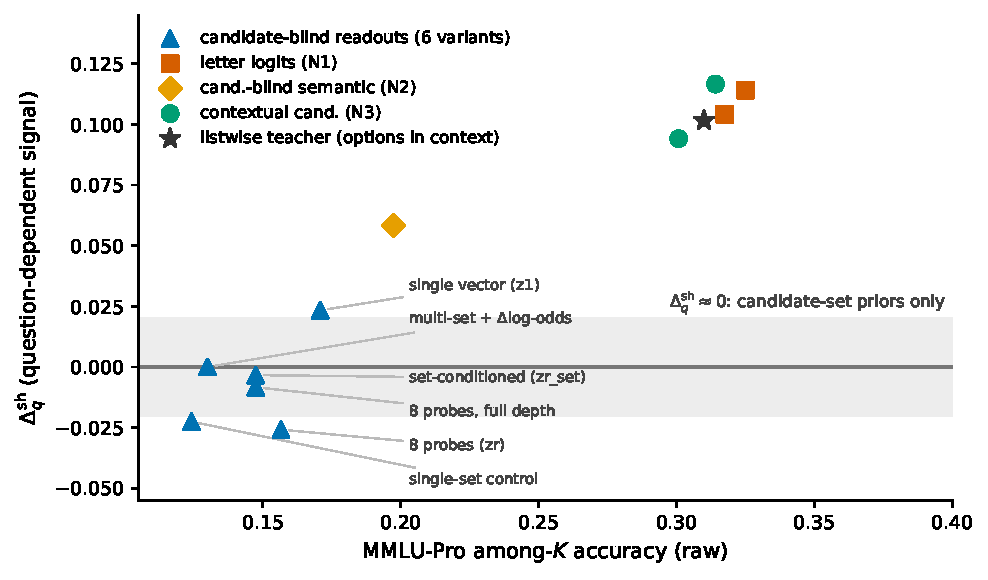
\includegraphics[width=\linewidth]{figures/fig_deltaq.pdf}
    \caption{MMLU-Pro among-$\numcands$ accuracy against $\dqsh$ ($n{=}1{,}200$; shaded: the $\pm.02$
    band). The six candidate-blind variants cluster at zero; N1, N3 and the teacher carry
    .09--.12.}
    \label{fig:deltaq}
  \end{minipage}
\end{figure}

\subsection{The evidence}
\label{sec:analysis:depth}

The decision should change when the evidence changes. Two designs failed this test in different places,
one in the architecture and one in the training data. The first full-scale model in this project read
the last layer and scored 58.6 on SNLI, the score of a baseline that never sees the premise
(\Cref{app:extra-figures}). Comparing against that hypothesis-only baseline is what exposed
it. Reading at 71\% of depth gives one model that carries both evidence reasoning and question-conditioned
knowledge. With head, data and steps fixed, reading N3 at layer 20 instead of 28 raises
SNLI/MNLI/ANLI/BoolQ from .863/.752/.431/.737 to .906/.865/.519/.834 while $\dqsh$ stays at .118
against .117 (CLINC-150 and validation NLL in \Cref{app:extra-figures}). Evidence accuracy
lands within 1--4 points of a candidate-blind energy-scoring baseline on every evidence set and 8 points above it on CLINC-150, so one model serves the evidence and knowledge regimes that
had needed separate models. For a candidate-blind state the same change moves nothing on $\dqsh$, and its evidence accuracy
regresses at full depth (\Cref{tab:app-blind-closure}).

\label{sec:results:long}
The second failure sat in the long-document training data. Training right-truncates states at the
window, and the long-state corpus rendered the case facts after the policy text, so at 1{,}024 tokens
the facts were lost in 98.8\% of long-policy rows (\Cref{sec:train:long}). The test that exposed the defect is a render-crossed
$2\times2$. Two 1.7B arms with byte-identical flags train on the same 23{,}318 rows, rendered
facts-first or facts-last, with truncation active as at release, and are scored under both renders
(\Cref{tab:twobytwo}) on 605 held-out long states, never truncated at evaluation, that differ only in
where the evidence sits (\Cref{app:truncation}). The comparison is a \emph{matched-configuration gap}:
each model is scored in the render it was trained on, so the evaluation render changes along with
training.

\begin{table}[t]
  \centering
  \caption{Training render $\times$ evaluation render on 605 held-out long states, no truncation at
  evaluation. Diagonal (matched) cells score each model in its training render; off-diagonal cells hold
  the evaluation render fixed across the two models. Floors and sizes in \Cref{app:protocol}. 14B arms:
  \texttt{tl1b\_nokd} (facts-first) and \texttt{ladder\_14b} (facts-last).}
  \label{tab:twobytwo}
  \footnotesize
  \setlength{\tabcolsep}{4pt}
  \begin{tabular}{llrrrrrr}
    \toprule
    & & \multicolumn{3}{c}{1.7B, single-variable (seed 0)} & \multicolumn{3}{c}{14B corroboration} \\
    \cmidrule(lr){3-5}\cmidrule(lr){6-8}
    Trained on & Scored on & overall & permit & select & overall & permit & select \\
    \midrule
    facts-first & facts-first \emph{(matched)} & \textbf{.942} & \textbf{.933} & \textbf{.953} & \textbf{.997} & .997 & .996 \\
    facts-first & facts-last & .797 & .788 & .807 & .921 & .933 & .905 \\
    facts-last & facts-first & .640 & .615 & .669 & .851 & .839 & .865 \\
    facts-last & facts-last \emph{(matched)} & .830 & .842 & .815 & .919 & .930 & .905 \\
    \bottomrule
  \end{tabular}
\end{table}

Training with the evidence placed first adds 11.2 points on held-out long states when training
right-truncates states at 1{,}024 tokens, and the gap replicates at a second seed. At 1.7B the
matched-configuration gap is $+.112$ $[+.077, +.147]$, $p = 5\times10^{-10}$, and a second seed of the
whole pair gives $+.111$ (.937 vs.\ .826), with every cell within two points of seed 0. At 14B the gap
is $+.078$ $[+.055, +.100]$, $p = 7\times10^{-12}$, smaller because the facts-first model is at ceiling
(.997). The two 14B checkpoints differ in the rest of the recipe bundle as well, so the 14B pair
corroborates the direction at scale and the 1.7B pair is the single-variable test. The v2 releases carry
the fix: on facts-first long states they score .947 (1.7B) and .950 (4B) against .598 and .612 for v1,
and hold their facts-last accuracy (\Cref{tab:app-long-release}).

JevBench does not register the change (\Cref{app:truncation}): its 19-item \texttt{long\_policy}
family gives 6/19 against 2/19 ($p = .232$) at one seed and 5/19 against 5/19 at the other
(\Cref{app:hard-tier}). The purpose-built 605-item set resolved at $p < 10^{-9}$ what a 19-item
benchmark cell could not, and before the fix benchmark gains and the defect coexisted
(\Cref{app:mixture}). The off-diagonal cells of \Cref{tab:twobytwo} hold the
evaluation render fixed; they measure a dependence on layout, which \Cref{sec:results:rendering} takes up.

\subsection{The rubric}
\label{sec:results:mixture}

The decision should change when the rubric changes. Workflow decisions arrive with a rubric that says how
to decide, and nothing in ordinary training data forces a model to read it: when each state appears under a
single rubric, the state and candidates can carry the answer on their own. A model never trained on the
generator shows the cost on held-out families, grammars and rubric styles, where it scores
.481/.507/.491, and on held-out rubric-flip pairs, where the same state and candidates take a different
gold under a different rubric, it scores .477. All comparisons in this subsection and in
\Cref{sec:analysis:null} are matched 1.7B runs that differ only in data or sampler.

The fix is in the data. DecisionMix v2 (\Cref{sec:train:rubric}) builds every row into a counterfactual
rubric group: the same state and candidate set under at least two rubrics with distinct gold answers. A
predictor that ignores the rubric assigns one distribution to every member of a group, so on a
two-member group its average cross-entropy stays at or above $\log 2$ nats, and the loss falls below
that floor only by reading the rubric. Held-out compositions,
domains, styles and grammars stay evaluation-only, and level 7 (temporal, numeric, probability and
trade-off composition) never enters training, so the test measures rubric reading on groups the model
never saw (\Cref{app:corpora}).

Training on DecisionMix v2 lifts held-out families, grammars and rubric styles by 35--40 points over a
model never trained on the generator (.481/.507/.491 $\to$ .827/.881/.888, together with the uncertainty
corpus), and accuracy on held-out rubric-flip pairs from .477 to .710; the model now depends on the
rubric it is given (\Cref{app:decisionmix}). The shuffled-rubric control agrees: accuracy under a
shuffled rubric falls from .446 to .405, so a wrong rubric now costs the model answers. The treatment
also changed the sampler, the gains are measured within the generator's own rule engine, level-7
composition moves only from .477 to .498 (\Cref{sec:limitations}), and the original workflow sets give
up 3--5 points (\Cref{app:decisionmix}).
